\section{Signature for Sequential Circuit}


In this section, I discussed the signature for two sequential circuits, i.e., 3-bit counter and FIR filter

\subsection{3-bit Counter}


Figure~\ref{fig:matlab} shows the 3-bit counter in MATALB Simulink. I have derived the signature by Stuck-at-fault model to different all possible nodes. Table~\ref{s@1-O0}  shows the signature values if the node B0 stuck at "1." Similarly, I have derive the signatures for all the nodes.



\begin{figure}
 \centering
  \captionsetup{justification=centering}    
   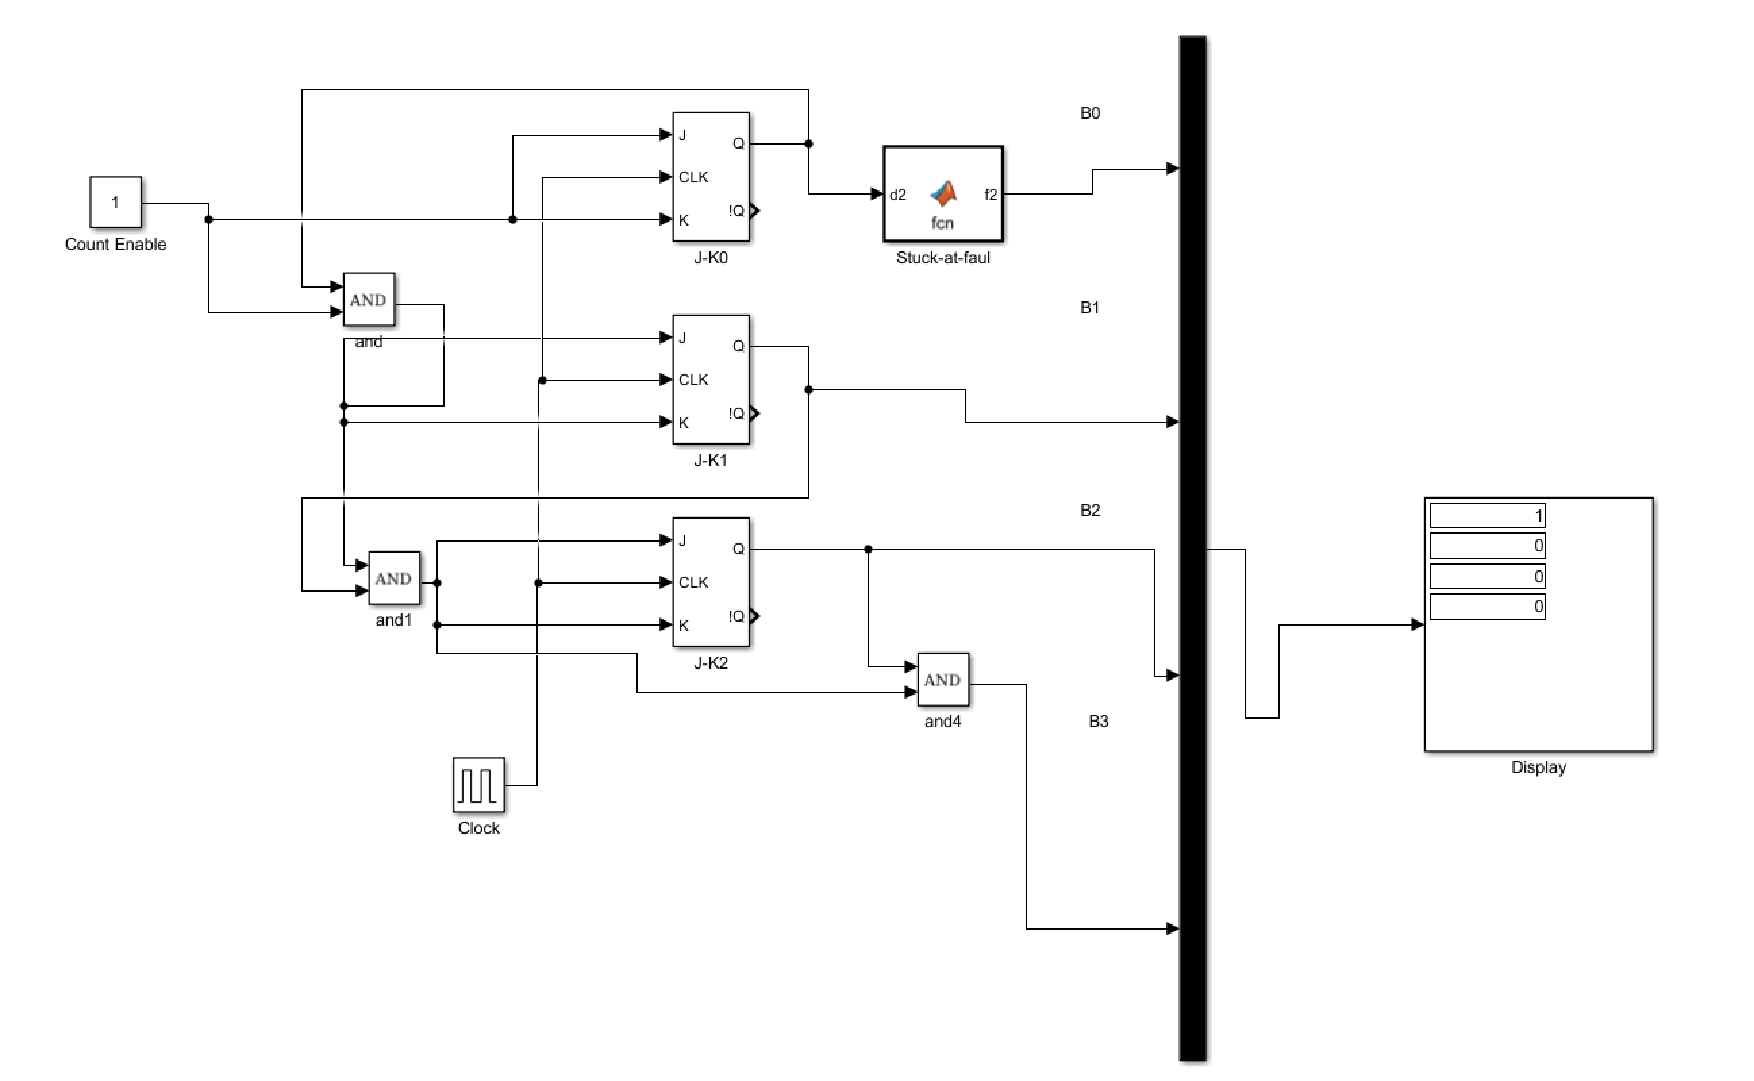
\includegraphics[scale=0.4]{Figures/matlab-counter.pdf}
   \caption{3-bit counter in MATALB}.
\label{fig:matlab}
\end{figure}


\begin{table}[tb!]
\center
\caption{Stuck-at-1$\rightarrow O_0$}

\label{s@1-O0}

\begin{tabular}{|c | c| c | c| } 
 \hline
 \rowcolor{lightgray}
Faulty Value (Binary) & Faulty Value & Original Value & Arithmetic Signature   \\ 
\hline
 
 
 001& 1 &0 & -1  \\
 \hline
 011 & 3 & 1 & -2 \\ 
 \hline
 
 101 & 5 & 2 & -3 \\
 \hline
 111& 7& 3& -4 \\
 \hline
 001 & 1  &  4& 3 \\
 \hline
 011 & 3 & 5 &2  \\
 \hline
 101 & 5 & 6 & 1 \\
 \hline
 111 & 7 & 7 & 0 \\
 \hline
 
 
\end{tabular}
\end{table}



\section{Signature for FIR Filter}
